

% Hasonló rendszerek
% https://esphome.io/
% https://www.openhab.org/
% Kész termékek
% https://www.itead.cc/sonoff-pow.html

%mqtt https://ieeexplore.ieee.org/abstract/document/4554519
%smarthome + nodered https://ieeexplore.ieee.org/document/8603575
%titkosítások összehasonlítása https://ieeexplore.ieee.org/abstract/document/8822208

\chapter{Felhasznált technológiák}
\section{ESP8266}
Az egységek alapja egy az Espressif cég által gyártott mikrokontroller, amelyen található egy 32bit-es 80Mhz-es Tensilica processzor, 50kB RAM, egy külső flash chip. Az utóbbi flash felelős felhasználói program tárolásért. Emellett megvalósításra került egy teljes WiFi stack-et, amely támogatja a 802.11 b/g/n szabványokat. A modulnak két virtuális WiFi interfésze van, amikkel tudja biztosítani, hogy állomásként (station), elérési pontként (softAP) vagy egyszerre mind a két módon üzemeljen. Az utóbbi tulajdonság segítségével lehet Mesh hálózatokat létrehozni.

\begin{figure}[!ht]
    \centering
    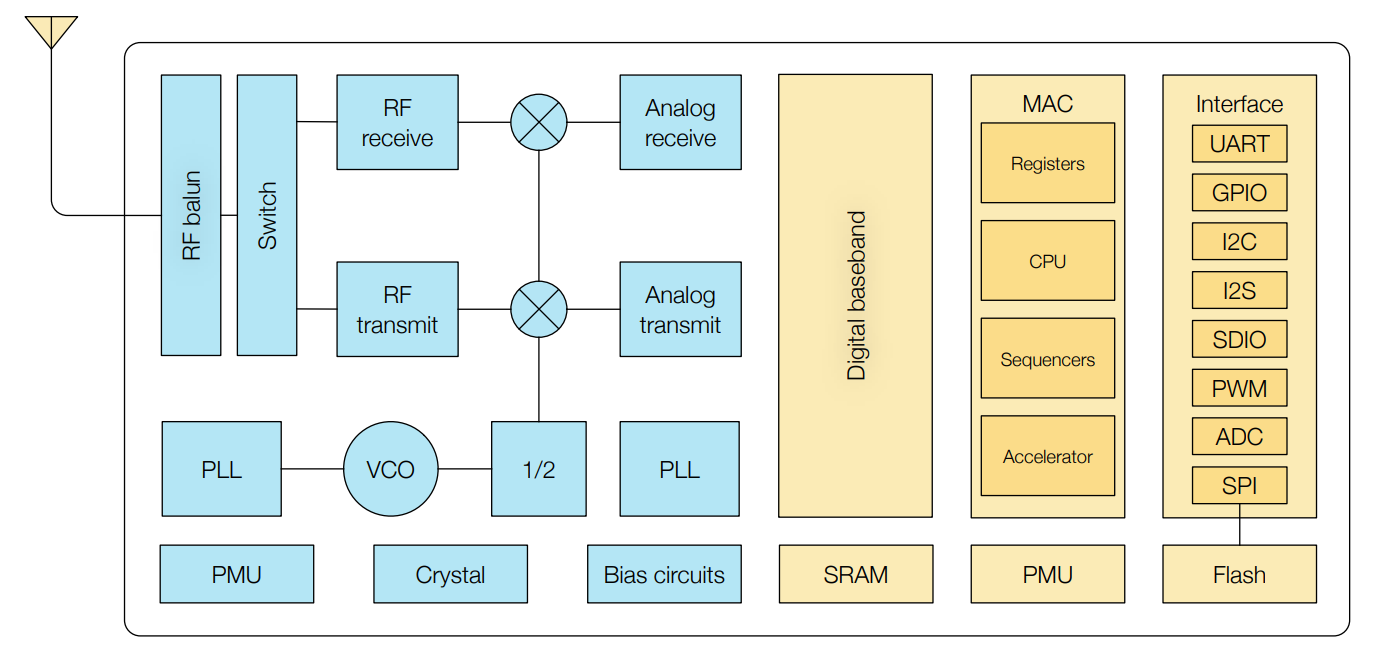
\includegraphics[width=150mm, keepaspectratio]{figures/esp8266funcdiag.png}
    \caption{Az ESP8266 funkcionális diagramja}
    \label{fig:TeXstudio}
\end{figure}

A ESP8266-hoz léteznek különböző típusú moduljai (pl. ESP-01, ESP-12). Az eltérés a modulok között általában a panelre kivezetett GPIO szám és a modul mérete jelenti. Összesen 17 db GPIO láb áll rendelkezésre, amelyekhez különböző funkciók rendelhetők. Szoftveresen beállítható egy kivételével mindegyik lábra interupt. Rendelkezik 2db UART, 3db SPI és szoftveresen beállítható I2C interfésszel is.
Az IoT rendszerekben és távol vezérlésű rendszerekben népszerűen használják, ami elsősorban az alacsony árának és a vele kompatibilis fejlesztői környezetnek (pl. Arduino, VStudio) is köszönhető. Rengeteg előre elkészített könyvtár található hozzá, amikkel gyorsan lehet például prototípusokat elkészíteni. A gyártó alapvetően 3 különböző SDK-t biztosít a fejlesztéshez. Az Arduino core-t, NONOS SDK-t, illetve a RTOS SDK-t. Az utóbbi egy FreeRTOS alapú operációs rendszer.

Számos versenytársa létezik például a RTL8710, AIR602 amik eltérő processzort használnak, de alapvető tulajdonságaikban nincs nagy eltérés. ezenkívül létezik már az 8266-nak egy újabb verziója az ESP32, ami már 2-magos processzorral, nagyobb memóriával és több perifériával rendelkezik.

% http://wiki.seeedstudio.com/W600_Module/
% különböző modul típusok
% elérhető lábszám
% alacsony ár
% miben lehet rá fejleszteni
% iotban elterjedt, hasonló ellenfele RTL8710


\section{ESPNOW}
Az ESPNOW egy kommunikációs protokoll, ami WiFi-hez hasonlóan a 802.11-es szabvány alapján működik. Az egyik eltérés a WiFi-hez képest, hogy nincs külön kapcsolat felépítés az eszközök között. Ennek köszönhetően kevesebb az overhead a kommunikáció során, és így kissebek az átküldött csomagok mérete.

A fizikai és hozzáférési réteg felett a gyártó által definiált egyedi keret található. A frame tartalmaz egy Body mezőt, ami tartalmazhatja az alkalmazásunk payload-ját. Ennek a mérete 0-250 byte között változhat. A keret ezenkívül tartalmaz még számos a gyártó által használt mezőt, mint pl ESPNOW verziószámát, egyedi azonosítót, ami az adott ESP MAC címének az első 3 bájtja alkot.

\begin{table}[ht]
	\footnotesize
	\centering
	\begin{tabular}{ | c | c | c | c | c | c |}
		\toprule
		Egység ID & Méret & Azonosító & Típus & Verzió & Body \\
		\midrule
        1 bájt & 1 bájt & 3 bájt & 1 bájt & 1 bájt & 0-250 bájt \\
	\end{tabular}
	\caption{ESPNOW keretformátum}
	\label{tab:TabularExample}
\end{table}

Az adatküldés előtt az egységeket párosítani kell egymáshoz. Ez az inicializálás során történhet meg egyszerűen a másik eszköz softAP interfészének MAC címét megadva. Lehetség van tovább broadcast üzeneteket is küldeni az azonos csatornán lévő eszközöknek. Ebben az esetben a párosítás során a broadcast FF:FF:FF:FF:FF:FF címet is hozzá kell adni. Lehetőség van a 2.4ghz sávban található 14db WiFi csatorna használatára. Egy modul maximum 20 másik eszközzel lehet összepárosítva. Lehetőség van továbbá a kiküldött keretek titkosítására is ez AES-128 algoritmus használatval történik. 
Az ESPNOW által küldött üzenet a SoftAP interfészén keresztül történik, viszont az AP interfész ettől függetlenül tud kapcsolódni más WiFi hozzáférési pontra. Ez a megoldás annyi megkötéssel tud működni, hogy ugyanazt a csatornát kell használi mind a két inferfészén. Létrehozható így könnyen egy átjáró az ESPNOW hálózatunk és az internet között plusz eszköz használata nélkül.

% nincs külön kapcsolat két eszköz között
% custom frame format
% sikeres küldés esetén ack, TODO mérni kellene
% https://docs.espressif.com/projects/esp-idf/en/latest/api-reference/network/esp_now.html

% https://cr.yp.to/chacha/chacha-20080128.pdf
% https://cr.yp.to/snuffle/salsafamily-20071225.pdf
\section{ChaCha}
A titkosítás egy 256 bites kulcson alapul és alapvetően a Salsa20-as algoritmus egy tovább fejlesztett változata. Mind a két algoritmus szimmetrikus kulcsot használ és folyamatosan rejtjeleznek, nem blokkonként. Az említett algoritmusok egyik nagy előnye, hogy csak három művelet ismételődik. Ezek a műveletek az összeadás, kizáró vagy és az elforgatás. A bemenetek 32 bites számoknak tekinthetőek. A titkosítás alapja egy 4x4-es mátrix, aminek elemei a 32 bites értékek. A mátrixot a 4 db bemeneti adat, 8db kulcsérték, 2 db számláló és 2db noonce érték alkotja.

\begin{table}[h]
	\footnotesize
	\centering
	\begin{tabular}{ c c c c }
		Adat & Adat & Adat & Adat \\
		Kulcs & Kulcs & Kulcs & Kulcs \\
		Kulcs & Kulcs & Kulcs & Kulcs \\
		Számláló & Számláló & Nonce & Nonce \\
	\end{tabular}
	\caption{ChaCha mátrix felépítése}
	\label{tab:TabularExample}
\end{table}

Az egyszerű műveletek használata miatt egyszerűen implementálható és jól használható kis teljesítményű processzorok esetében is. Beágyazott környezetekben szintén elterjedten használják, az előbb említett tulajdonság miatt is, illetve mivel a rejtjelezés helyben végezhető. A szintén sok helyen használt AES-hez képest gyorsabb és hasonlóan biztonságosnak tekinthető.

\section{MQTT}
Az MQTT publikáló-feliratkozó modell alapján működik. A klienseknek lehetőségük vannak különböző topikokra feliratkozni, illetve saját topikokat is létrehozni és oda adatot küldeni. A működésük alapján a klienseket általában két csoportba oszthatóak. Léteznek olyan egységek, amelyek működésük során csak adatokat töltenek fel. Ezeket hívjuk publikáló egységeknek. A másik típusú egységek valamilyen téma-hoz tartozó adatot figyelnek és az alapján döntenek. Ezek pedig feliratkozó típusú egységek. A rendszer központját egy bróker alkotja, aki biztosítja, hogy az egységek tudjanak üzenetet küldeni és fogadni.

\begin{figure}[!ht]
    \centering
    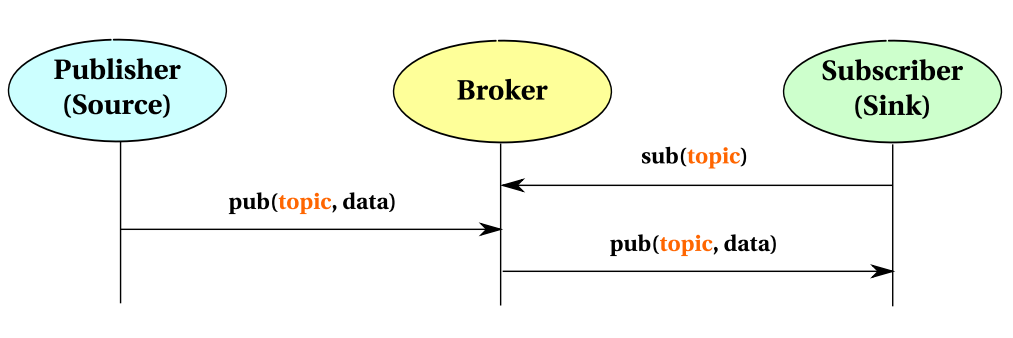
\includegraphics[width=130mm, keepaspectratio]{figures/mqtt.png}
    \caption{MQTT protokoll működése  \cite{MQTTS—Ap4:online} }
    \label{fig:mqtt}
\end{figure}

Az eszököz kommunikációja TCP/IP felett zajlik. A protokollban használt csomagok három fő részből állnak össze. Mindegyik üzenet tartalmaz egy fix 2 bájt méretű részt, amiben megjelenik többek között a csomag típusa és méretét. Ezt követhet egy opcionális fejléc, amit csak bizonyos típusú csomagok használnak. Ebben a fejlécben két bájton jelenik meg az adott típusú üzenet által definiált paraméterek, amik lehetnek például csomagazonosítók, vagy különböző visszajelző értékek. Az üzenet utolsó része pedig szintén opcionális és parancstípusától függ.Itt lehet megadni az üzenethez tartozó adatcsomagot.


\begin{table}[ht]
	\footnotesize
	\centering
	\begin{tabular}{|c|}
		\hline
		Fix fejléc, minden esetben létezik \\
		\hline
		Változó fejléc, csak bizonyos típusú MQTT üzeneteknél \\
		\hline
		Adatcsomag, csak bizonyos típusú MQTT üzeneteknél\\
		\hline
	\end{tabular}
	\caption{MQTT csomag felépítése}
	\label{tab:mqtt_package_format}
\end{table}


Az MQTT protokoll könnyű implementálhatósága miatt, az alacsony hálózati forgaloma és közel valósidejűsége miatt ideális választos különböző IoT-s rendszerek használatlánál. Egyedül a bróker futtatáshoz lehet szükséges nagyobb kapacitás, de számos cég biztosít lehetőséget ilyen szolgáltatások előfizetésére. Egy otthoni rendszer esetében elegenedő lehet például egy Raspberry PI-n futó szerver használata is. Az otthoni szerver használatának további előnye, hogy biztonságosabb rendszer hozható létre, mivel nem jutnak ki a szenzor információk az internetre.

\section{Node-RED}
A Node-RED egy olyan programozási felület, amely segítségével könnyedén összelehet kapcsolni különböző internetes szolgáltatásokat, hardveres eszközöket. A felület futattásához szükséges egy szerver, ami lehet például egy lokálisan elhelyezett Raspberry PI-n. Egy másik lehetséges megoldás a különböző cégek által biztosított felhőalap rendszerekben történő futtatás.

A rendszert futtató szerver NodeJS-ben lett elkészítve, amelynek az egyik fő jellemzője, hogy könnyen lehet párhuzamosan futtatni különböző feladatokat. További előnyeihez sorolható, hogy a rendszer nyílt forráskódú és felhasználóknak lehetőségük van saját kiegészítők készítésére.

A programozási felülete alapvetően egy grafikus felület, amin különböző blokkok helyezhetők el, és ezeket lehet összekötni különböző módokon az elvárt működésekhez. Az alkalmazás használáshoz programozási előismeretek nélkül is könnyedén használható a felhasználók számára. Lehetőség van ezenkívűl javascript nyelven megírt kódrészletek használata is.

\begin{figure}[!ht]
    \centering
    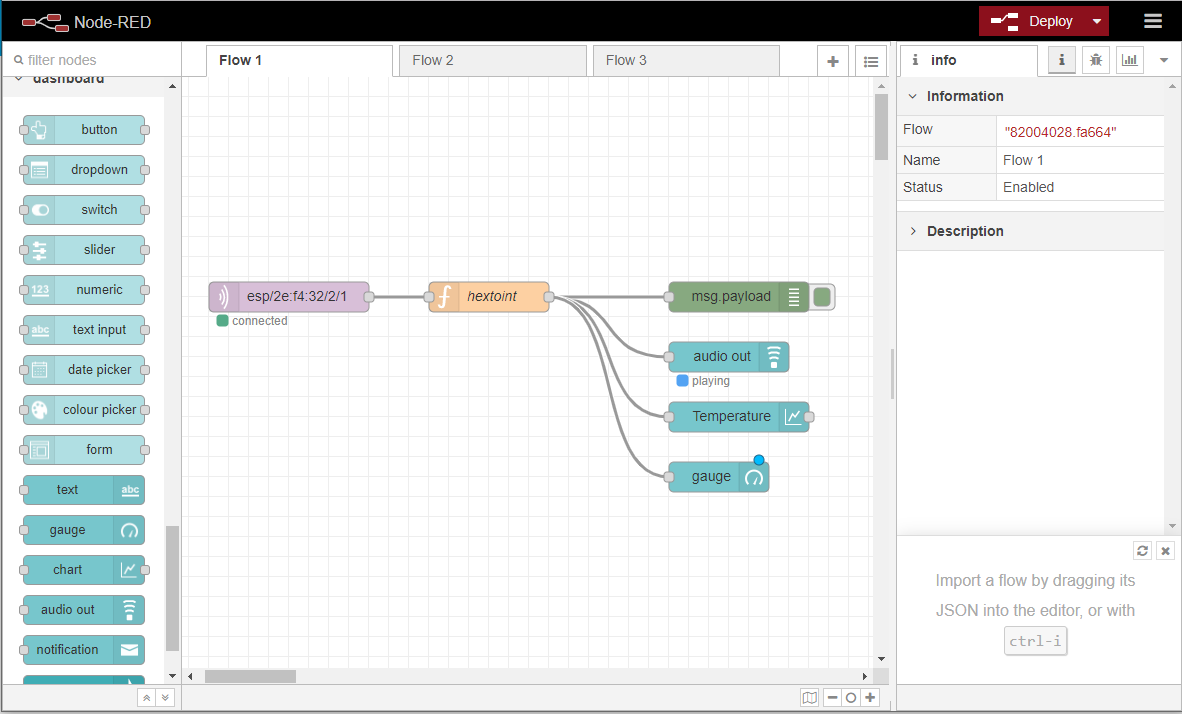
\includegraphics[width=150mm, keepaspectratio]{figures/nodered.png}
    \caption{Node-RED fejlesztői felület}
    \label{fig:nodered_development}
\end{figure}

A felület 3 fő részre különíthető el. A baloldalon találhatók a feltelepített könyvtárakban található blokkkok. A középső részben tudjuk konkrétan a kapcsolatokat létrehozni, a jobb oldalon pedig az egyes blokkok tulajdonságai módosíthatók. A fejlesztői környezeten lehetséges saját nézeteket is létrehozni a felhasználóknak. Ezeknek a felületeknek egy fontos jellemzője, hogy reszponzívak, tehát könnyen haszálhatók kis kijelző mérető eszközökön, például telefonokon is.

\begin{figure}[t!]
    \centering
    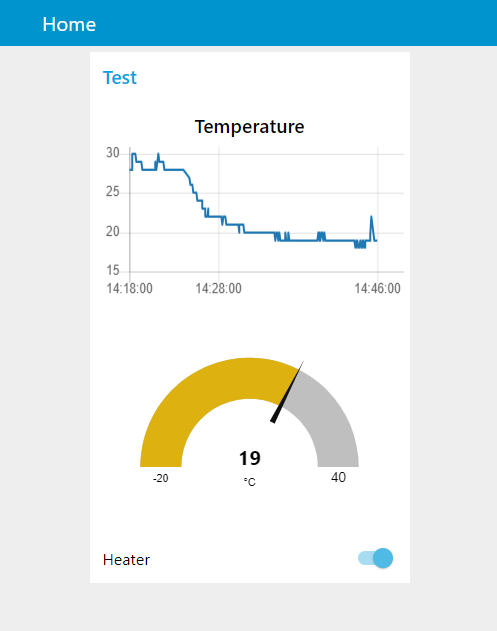
\includegraphics[width=90mm, keepaspectratio]{figures/nodered-ui.png}
    \caption{Node-RED felhasználói nézete}
    \label{fig:nodered_ui}
\end{figure}

A \ref{fig:nodered_development} és \ref{fig:nodered_ui} képeken például egy MQTT protokollt használó egység hőmérséklet szenzor értékei vannak megjelenítve. Illetve lehetősége van a felhasználónak bekapcsolni a fűtegységet szintén egy MQTT csomag küldése segítésgével.

% https://nodered.org/
